
\chapter{Creating the initial simulation with Flutter}

Flutter was used for the initial simulation due to prior knowledge of the framework. I chose it because I knew I was going to get things wrong, and I wanted to at least partly be in a familiar environment while understanding reaction diffusion. 

See Figure \ref{fig:first-waves} for a picture of the first successful waves. 

\subsection{Why Flutter was a good choice for the initial simulation}

\begin{enumerate}
    \item \textbf{Prior framework knowledge}: I have worked with this framework for several years and I am very comfortable with this. I used it to my advantage to reduce the number of unknowns in the initial stage of the project. 
    \item \textbf{Pixel-level control}: Flutter can jump down to pixel-level operations at any time. 
    \item \textbf{Fast prototyping}: Flutter is known to be very fast for prototyping initial designs and I used that to quickly create a simulation without much commitment
\end{enumerate}

In this project I used a \verb|CustomPainter| and a `dart:ui` Image, a snipped of the code is available in Figure \ref{fig:flutter-painted-code}. 


\begin{figure}
    \centering
\begin{verbatim}
AspectRatio(
  aspectRatio: _imageData!.width / _imageData!.height,
  child: CustomPaint(
    size: Size(
        image.width.toDouble(), image.height.toDouble(),
    ),
    painter: ReactionDiffusionPainter(_imageData!),
  ),
),
\end{verbatim}
    \caption{Snapshot of Flutter code used to render the simulation}
    \label{fig:flutter-painted-code}
\end{figure}


\subsection{Problems with using Flutter}

\subsubsection{Neumann Boundary Problem}
I ran into several issues with the rendering. In Figure \ref{fig:neumann-bondary} you can see how the edges of the picture were causing problems for the reaction. This is because the diffusion code uses all neighbours to calculate diffusion ??? what?? and the edges didn't have anything there, so they were causing issues. This was easily fixed by implementing that edge case and assuming everything is 0 there. 

\subsubsection{Bitmap Compression}
The original simulation I built using Flutter used integers and it worked partly, but there were problems, such as it was having difficulties getting out of low and high numbers when the timestep \verb|dt| was set to a low value like 0.0001. I discovered that this was because my code was using integer values and when the simulated timestep was very small, the update was less than 1, so it was getting rounded to 0. 
I really wanted to use integeres tho because they can be updated in place inside bitmaps and that speeds up everything massively. I tried integer compression using the following assumption:
Small Values: Small values (close to zero) change the output value significantly. This is crucial for your simulation where small changes matter.
Large Values: As values get larger, the rate of change in the compressed value decreases. This means that large values are represented with less precision, which is typically acceptable.
I was trying to quantities the results to fit in an uint8 variable in order to not have to update the bitmap every state, the bitmap is my state, this makes it more efficient. 
I used logarithmic quantisation for this and it did improve the simulation a little bit, but not as much as I expected. 
When I drew something onto the substrate in Figure \ref{fig:rounding-problem}, you can see how the reaction is not strong enough to reduce the activator chemical due to the integers used. 

To solve this problem I searched for file formats that supports floats like TIFF and I found that I can directly use an image library in flutter that doesn't go through file formats, but processes images directly like \verb|package:image| where I could directly declare the image as using the float format internally \verb|img.Image(width: width, height: height, format: img.Format.float64);| and since Flutter is Open Source I could verify the internals of the library and I saw it is using multiple channels for the floats until the rendering and it does not convert data to integers internally until the rendering part, which was what I wanted. It started to fade finally after going to floats as seen in Figure \ref{fig:after-int-fix}.

\subsubsection{Diffusion Not Happening}
For some reason the diffusion was not happening. I explored that by looking into every single component of the Oregonator model code I used and I plotted it in real time using the \verb|package:flutter_math_fork| package as seen in Figure \ref{fig:after-int-fix} and I was able to touch every pixel and see how the formula is affecting it in real time. Using this approach, I was finally able to see that the inhibitor (\verb|v|) was not following the activator properly, but I didn't know why. 
Later I found that there was an error in my formula where I had forgotten (TODO show the equation diff) the v (inhibitor) in the first equation. Using that, I was able to get waves as seen in Figure \ref{fig:first-waves}.


\begin{figure}
    \centering
    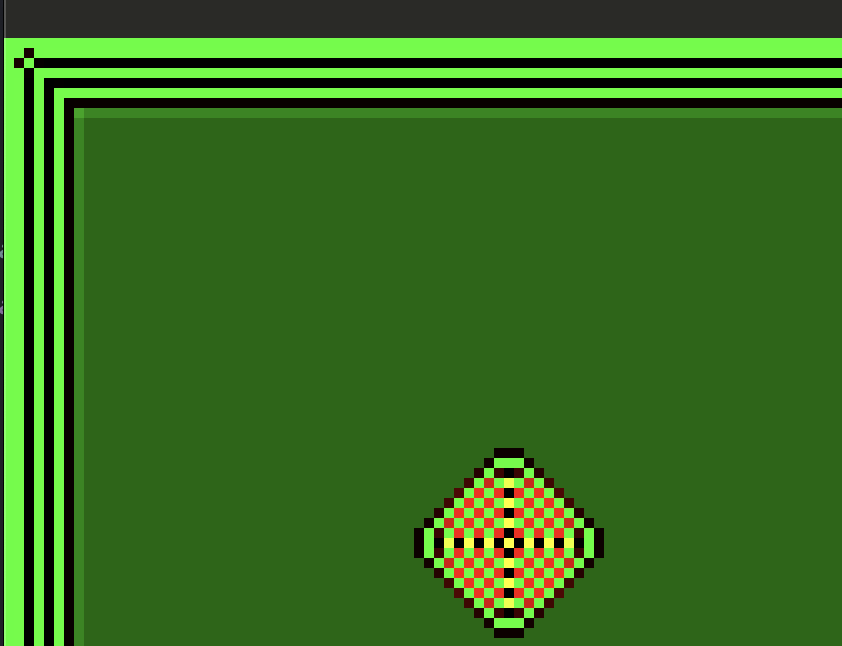
\includegraphics[width=0.5\linewidth]{neumann.png}
    \caption{Neumann Boundary Problem}
    \label{fig:neumann-bondary}
\end{figure}

\begin{figure}
    \centering
    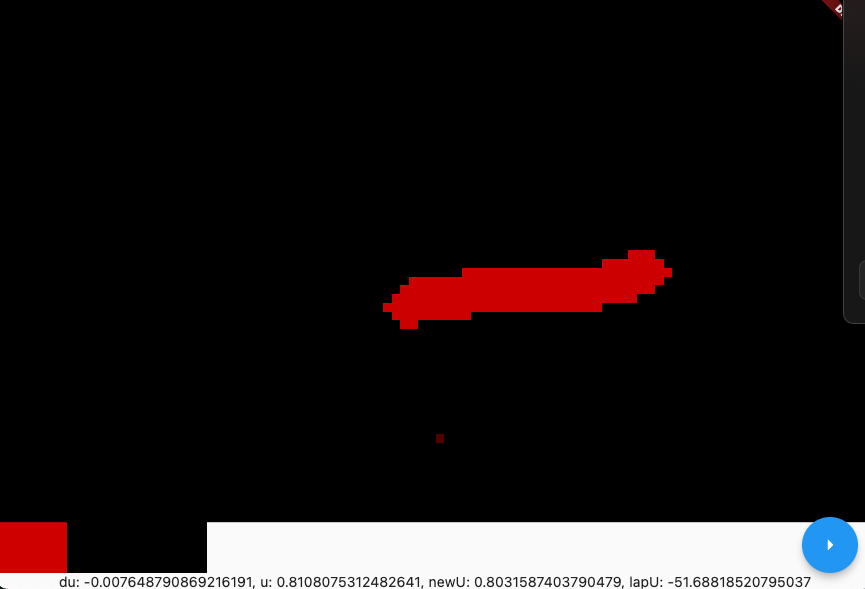
\includegraphics[width=0.5\linewidth]{int8.png}
    \caption{Rounding Problem in Flutter Simulation}
    \label{fig:rounding-problem}
\end{figure}

\begin{figure}
    \centering
    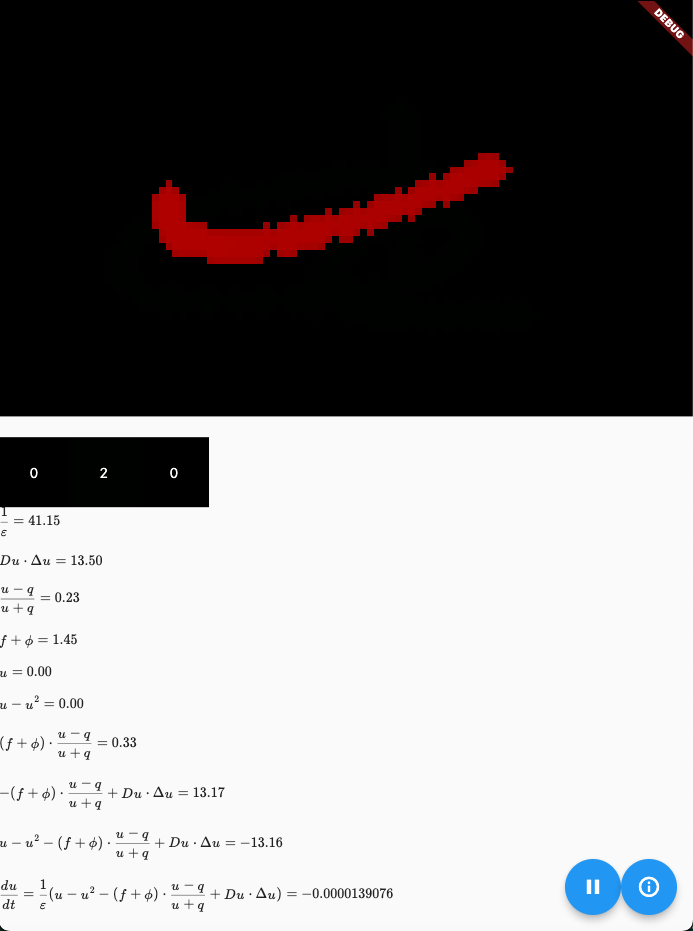
\includegraphics[width=0.5\linewidth]{after-int-fix.png}
    \caption{Finally started to fade after the switch to floats}
    \label{fig:after-int-fix}
\end{figure}

\subsubsection{Flutter GPU}
Flutter does not support GPU rendering as of February 9, 2024. This was necessary to speed up the simulation. I spent a lot of time getting the new \verb|package:flutter_gpu| internal package to work. 
New versions of the Flutter like \verb|3.16.0-0.5.pre| are compatible with latest versions of the Flutter Engine and I tried the latest versions to see if they expose such a package and they didn't publicly expose it. 
The person who currently works on the GPU part of the Flutter engine is Brandon DeRosier. I contacted him, but he never got back to me. I see him committing C++ code to the flutter engine, but it all looked partial and experimental, even though he has built GPU projects in Flutter with custom versions of the Flutter engine. Knowning that I built my own version of the flutter engine from the latest source code and try to expose the API myself. There is a public Google Document that describes the API for the Flutter GPU package: \verb|flutter.dev/go/impeller-dart|. 
I built my own version of the lastest Flutter Engine that was not released yet using. In this process I learned how to use custom Google tools like \verb|depot_tools| and \verb|gclient|, which is what Google uses as a wrapper for Git, etc. 
I built the engine for my M1 Mac using 

\begin{verbatim}
    ./flutter/tools/gn --unoptimized --mac-cpu=arm64
    ninja -C out/host_debug_unopt_arm64
\end{verbatim}

and I included it in the project with 
\begin{verbatim}
    flutter run --local-engine-src-path ../engine --local-engine=host_debug_unopt_arm64
\end{verbatim}

Even then, I was still not able to access the new Flutter GPU code. Looking further into the engine code. I noted that most of it is in TODO and there are very few things wired up from the C++ to the dart side. I didn't want to give up on the GPU side, so in Chapter \ref{chap:metal} I will explore how I used the Metal library to run the code on the GPU.

\section{Using Metal For The GPU}\label{chap:metal}

In Figure \ref{fig:metal-dependency-pipline} the red circles represent the Compute Command Encoder and the yellow circles represent the Render Command Encoder.
The Render Command Encoder runs for every frame, and the Compute Command Encoder runs as much as possible in the time the Render Encoder does not.

